\chapter{Related Work}\label{related}

\section{Projekte mit automatisierten Legerobotern}
Die Automatisierung der Baubranche hat neben Faktoren wie Geschwindigkeit, Effizienz und Kostenreduzierung auch den Vorteil Bauprojekte an Orten zu realisieren, die für Menschen ungeeignet sind~\cite{Petersen2012}.
Dafür wurde unter anderem das Projekt \textit{TERMES} von Kirstin Petersen et al.\ konzipiert, mit welchem das Team, angelehnt an dem Verhalten von Termiten, einen Schwarm bodengebundener Roboter koordinieren, die zusammen Strukturen errichten~\cite{Petersen2012}.
Darüber hinaus stellen Kirstin Petersen et al.\ in einer anderen Veröffentlichung eine umfangreiche Übersicht von weiteren Projekten aus dem Bereich \textit{Collective Robotic Construction} vor~\cite{Petersen2019}.
Doch nicht nur vollautomatische Roboterschwärme haben das Ziel die Baubranche zu verändern.
Es gibt bereits etablierte Firmen, die semi-automatische Roboteranlagen zur Unterstützung der Arbeiter vor Ort anbieten und damit erfolgreich die Bauzeit reduzieren können.
Dazu zählt zum Beispiel \textit{Hadrian X} der Firma FBR:\ ein mobiler, bodengebundener Kran der in der Lage ist ausgehend von einem CAD Modell ein bis zu drei Stockwerke hohes Gebäude aufzuschichten~\cite{HadrianX}.
Ein weiteres Beispiel stellt \textit{SAM100}, ein mobiler Ziegelstein legender Roboter der Firma \textit{Construction Robotics} dar~\cite{SAM}.
Dieser kann sich sogar erhöht auf einem Gerüst bewegen.

\section{Planungsvorgehen}
Grundlage für sämtliche Projekte, in welchen mithilfe von Legerobotern automatisiert Gebäude beziehungsweise Gebilde mit einer Form von Bausteinen errichtet werden, ist eine vorangehende Planungsphase.
In dieser Planungsphase müssen die notwendigen Informationen zu allen benötigten Bausteinen gesammelt werden, um im Anschluss die Bauphase überhaupt zu ermöglichen.
Das sogennante \textit{Wall Detailing} stellt ein ähnliches Problem wie das \textit{3D Bin Packing Problem} dar und errechnet, ausgehend von einem 3D Modell eines Gebäudes und Informationen zu den gewünschten Mauerwerksverbänden und Bausteinformen, einen möglichen Bauplan für das gesamte Gebäude.
Unter dem \textit{Bin Packing Problem} (auf deutsch als Behälterproblem bekannt) versteht man das möglichst platzsparende Schichten von Objekten in einen oder mehrere limitierte Behälter.
Dies kann sowohl im zwei- als auch im dreidimensionalen Raum geschehen.
Besonders herausfordernd ist das Verteilen unregelmäßig geformter Objekte wie es etwa Xiao Liu et al.\ am Beispiel verschiedener geometrischer Formen oder Qiruyi Zuo et al.\ am Beispiel von Obstkisten zeigen~\cite{Liu2015}~\cite{Zuo2022}.
Während sich in diesem Bereich viel mit unregelmäßig geformten Objekten beschäftigt wird, kann im Falle von Wänden, die mit Bausteinen errichtet werden eine Einschränkung auf quaderförmige Objekte vorgenommen werden.
Zudem ist das Ziel des \textit{Wall Detailings} nicht eine möglichst gute, sprich eine möglichst lückenlose Lösung zu finden, sondern eine, die sinvoll aufgeschichtete Wände hervorbringt.
Dabei stellen vor allem Übergänge zwischen mehreren Wandstücken besonders kritische Bereiche dar, für die es vor Ort oft Expertenwissen benötigt.
Zusätzlich muss Mauerwerk in Deutschland und Europa einigen Normen entsprechen. 
Darauf wird in Kapitel~\ref{basics:Mauerwerksbau} näher eingegangen.
Nachfolgend werden einige Veröffentlichungen vorgestellt, die ein ähnliches Ziel wie diese Arbeit verfolgen.

\subsection{Digital Plan of Brickwork Layout for Robotic Bricklaying Technology}\label{related:digital_plan_of_brickwork_layout}
In diesem Paper stellen Usmanov et al.\ ein generelles Vorgehen für das Erstellen eines Ziegel-Legeplans für ein als digitales Modell vorliegendes Gebäude vor~\cite{Usmanov2021}.
Dieses Vorgehen gliedern sie in sechs Schritte:
\begin{enumerate}
\item Das vorliegende IFC Modell (siehe~\ref{basics:ifc}) nach Wandelementen durchsuchen und diese in das sogennante BREP-Format (siehe~\ref{basics:brep}) konvertieren.
\item Das Aufteilen des gesamten Modells in Schichten, die der Modulhöhe des verwendeten Ziegelsteinformats entspricht.
\item Verbindungen von getrennt modellierten Wandelementen heraussuchen. Dies ist zum Beispiel an Eckstücken der Fall, da dafür oft zwei einzelne Wandelemente modelliert werden, welche in einem Winkel zueinander stehen und sich berühren. Für die nachfolgenden Schritte sind diese Verbindungen relevante Informationen.
\item Mit den Informationen der vorhergegangenen Schritte können nun für jede Schicht kritische Bereiche identifiziert werden, an welchen später ein komplexer Legevorgang von Ziegeln von Nöten ist.
\item Nun werden zunächst die kritischen Bereiche anhand einer vorher definierten Legeanleitung mit teilweise angepassten Ziegelsteinen bestückt und im Anschluss die restlichen Bereiche aller Wände mit dem ausgewählten Standardziegel aufgefüllt. In diesem Schritt werden zusätzlich Fenster- und Türstürze über deren Öffnungen in den Wänden gelegt.
\item Dieser Schritt fasst das Anzeigen als 3D Modell und Konvertieren des Resultats in eine nicht konkreter definierte Listenform zusammen. Das Ergebnis für das von den Autoren ausgewählte Beispielgebäude ist in Abbildung~\ref{fig:related:usmanov} zu sehen.
\end{enumerate}

\begin{figure}[ht]
    \centering
    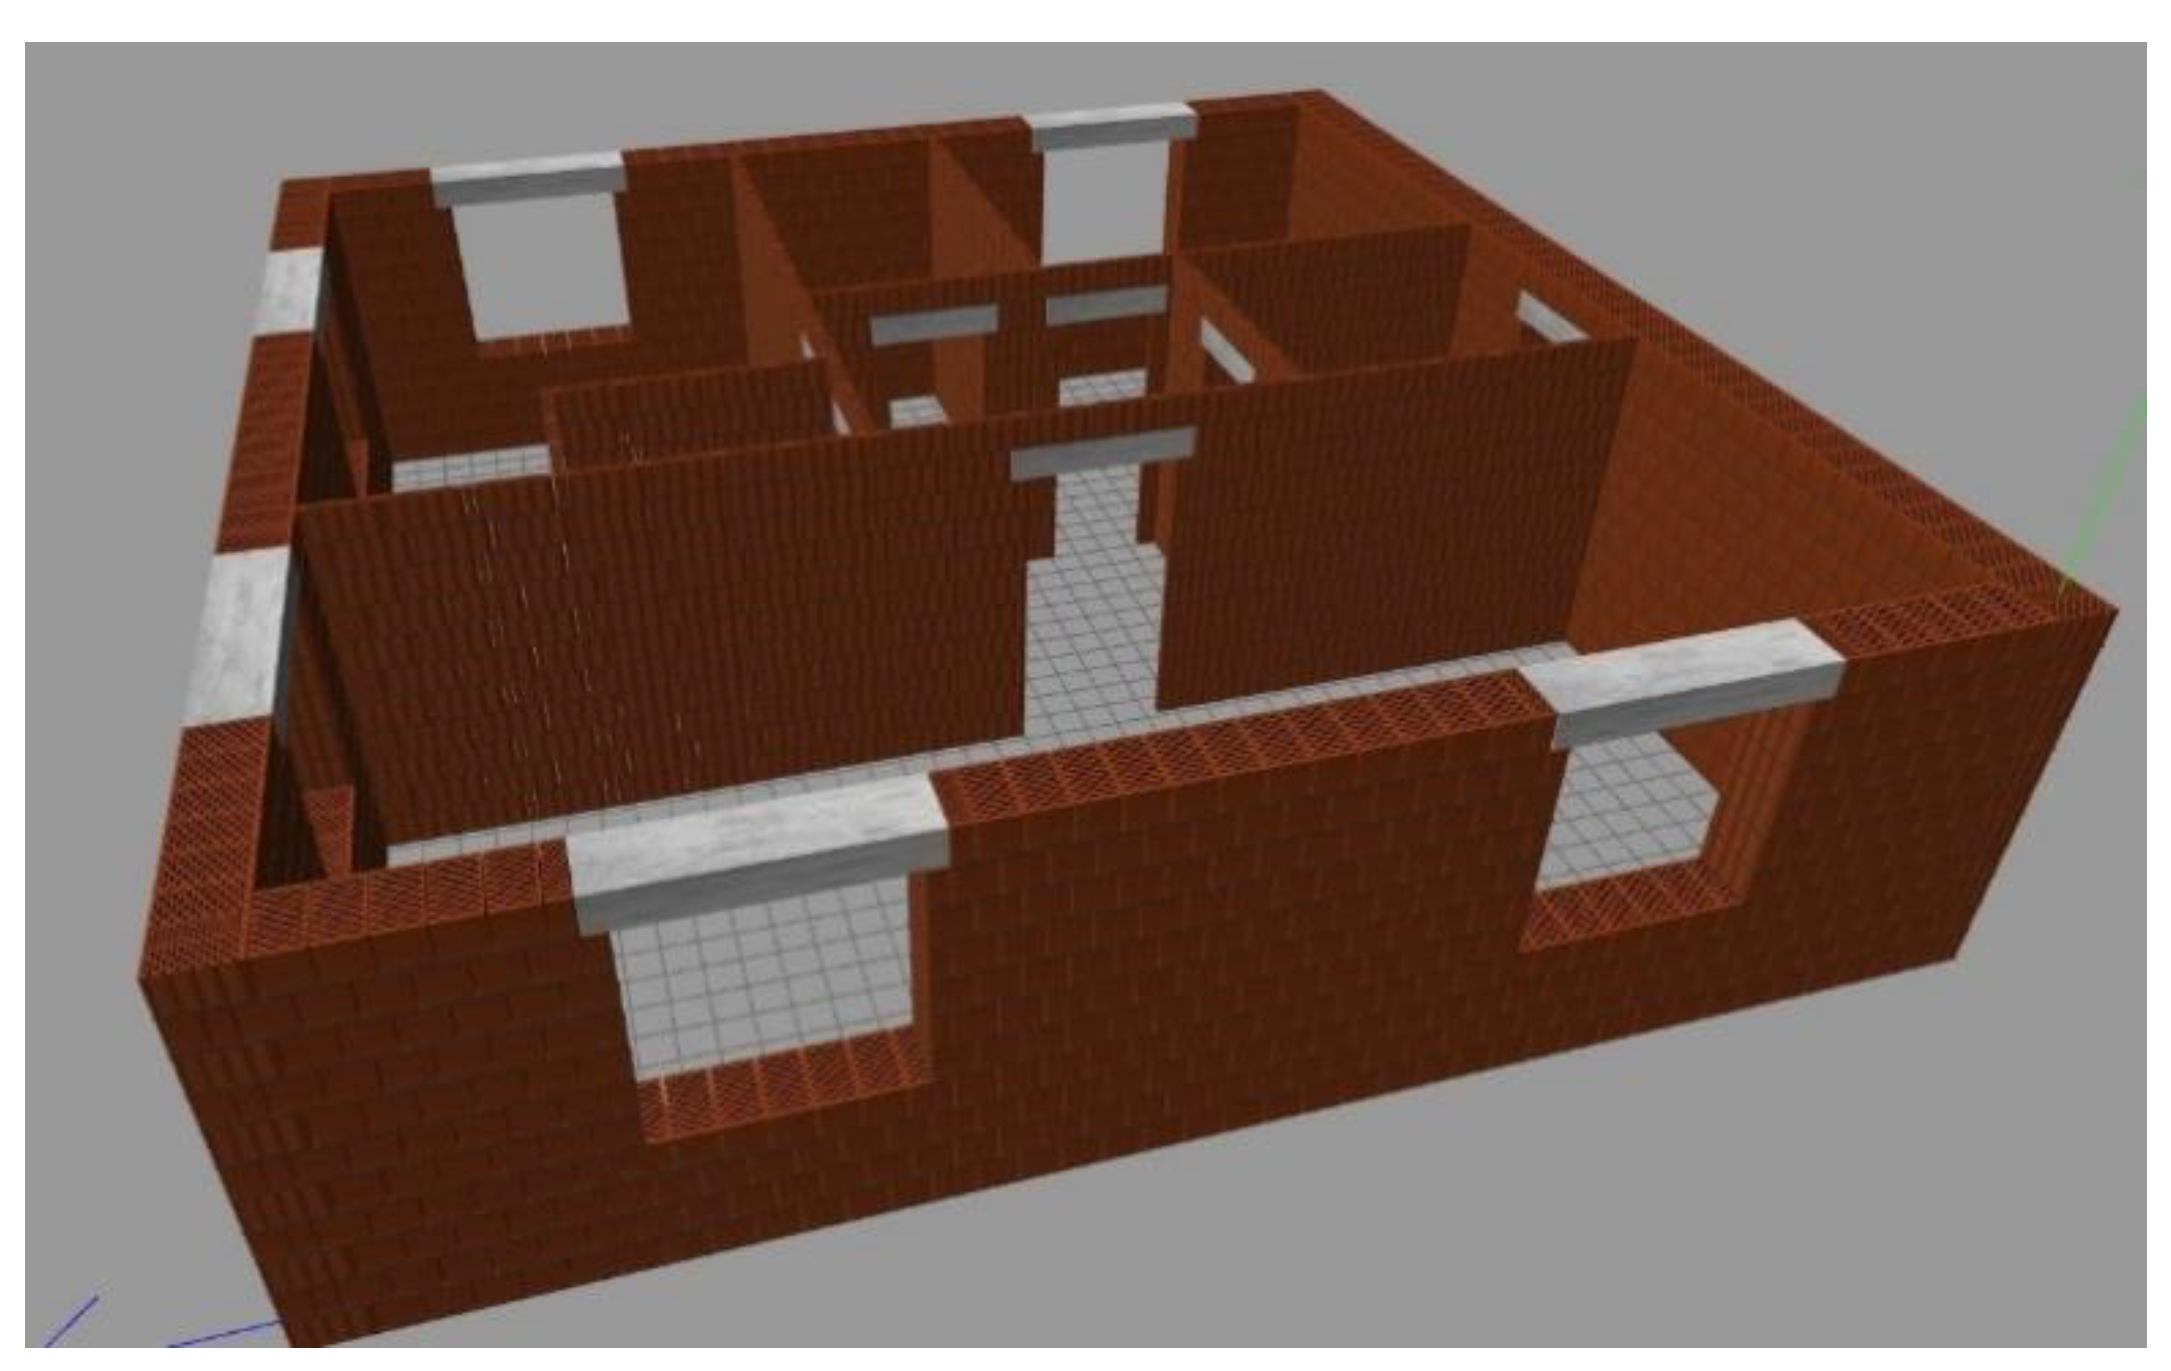
\includegraphics[width=0.6\columnwidth]{fig/sustainability-13-03905-g004.png}
    \caption{Ergebnis des Verfahrens zur Erstellung eines Ziegel-Legeplans nach Usmanov et al.~\cite{Usmanov2021}.}\label{fig:related:usmanov}
\end{figure}

Besonders detailliert ist ihr Ansatz für das Finden von besagten kritischen Teilbereichen einer Wand mithilfe mathematischer Gleichungen, die alle Wände zueinander in Beziehung stellen.
Diese Teilbereiche sind Wandecken, T-Kreuzungen (wie etwa der Übergang einer Innenwand an eine Außenwand) und Öffnungen innerhalb einer Wand und sind ebenfalls in Kapitel~\ref{scenarios:scenario2} dieser Arbeit als Fallbeispiel aufgeführt.
Anhand der von ihnen zusammengetragenen Informationen konnten die Autoren erfolgreich die bestmögliche Platzierung von vier Roboterarmen errechnen, die den schnellstmöglichen Bau des Gebäudes ermöglichen.
Dennoch werden zum Schluss noch einige Einschränkungen ihres Verfahrens angesprochen.
Vor allem die Beschränkung auf 90 Grad Ecken und das Gebunden sein an einen einzigen Standardziegel werden als besonders restriktiv wahrgenommen.

\subsection{Optimal brick layout of masonry walls based on intelligent evolutionary algorithm and building information modeling}
Xu Chengran et al.\ haben in ihrem Paper verschiedene Optimierungsansätze aus dem Bereich des 2D Packaging Problems getestet~\cite{Xu2021}.
%TODO was ist das für ein Problem? Zitat aus nem Paper finden!
Konkret wurden drei Algorithmen verwendet: Differential Evolution, Particle Swarm Optimization und Neighbourhood Field Optimization.
%TODO ergebnisse vergleichen und eines davon hervorheben, welches ich evtl selbst einbau
Außerdem wird ein drei-phasiges Vorgehen vorgeschlagen: Data collection, Brick layout und Data Output.
%TODO das vmtl einfach auch so aufziehen. Mauern aus modell extrahieren mit geometrischen infos, optimieren und iwie rausballern
Dieses Vorgehen eignet sich auch für das Finden von Bausteinkonfigurationen in dieser Arbeit, da zuerst alle relevanten geometrischen Daten (in diesem Fall Wände, Fenster, Türen usw.) aus dem 3D Modell gesammelt werden müssen, bevor das Detailing stattfinden kann.
Nach dem Optimieren der Bausteinkonfiguration muss das Ergebnis ebenfalls in ein Format gebracht werden, das für die folgenden Schritte verwendet und eventuell auch dem Nutzer angezeigt werden kann.

\subsection{Automated Brick Pattern Generator for Robotic Assembly using Machine Learning and Images}
Bárbara Andrade Zandavali et al.\ untersuchen in ihrem Paper wie gut sich Machine Learning Algorithmen dazu eignen anhand von Bildern Pläne für konkretes Mauerwerk zu erzeugen~\cite{Zandavali2019}.
Ein Kernaspekt dabei war das Anwenden verschiedener Mauerwerksverbände auf arbiträre Vielecke, welche die Form eines Wandabschnitts beschreiben.
\begin{figure}[hb!]
    \centering
    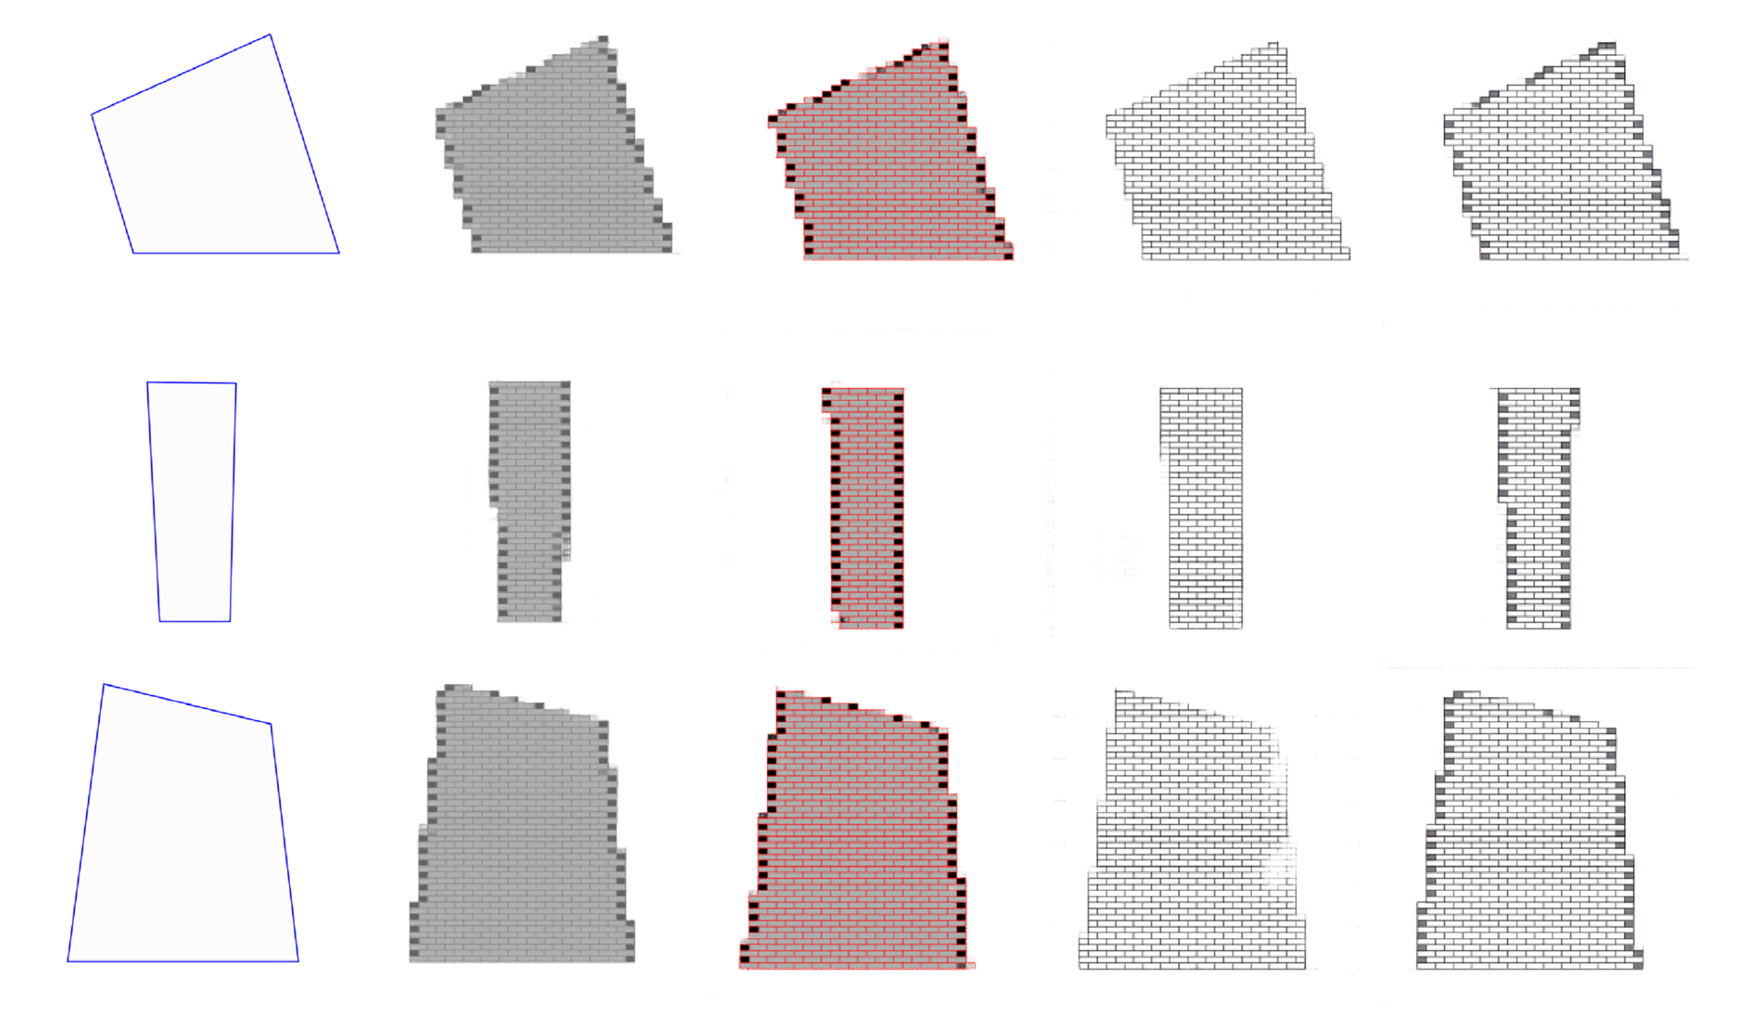
\includegraphics[width=0.8\columnwidth]{fig/ecaadesigradi2019_605.png}
    \caption{Eingaben und Ergebnisse des \textit{Brick Pattern Generator} nach Bárbara Andrade Zandavali et al.~\cite{Zandavali2019}.}\label{fig:related:Zandavali2019}
\end{figure}
In Abbildung~\ref{fig:related:Zandavali2019} sind verschiedene Eingabeformen (linke Spalte) und deren Ergebnisse in vier verschiedenen Ausgabearten zu sehen.
Da es sich sowohl bei dem Eingabe- als auch bei dem Ausgabeformat um Bilder handelt, musste im Anschluss zunächst untersucht werden, wie gut sich die verschiedenen Ergebnisarten dazu eignen daraus tatsächliches Mauerwerk zu interpretieren.
Zusammenfassend konnten die Autoren berichten, dass das Vorgehen teilweise zu fragwürdigen Resultaten geführt hat, welches sich aber mit Sicherheit noch verbessern lässt.
Dennoch ist der Anwendungsfall auf gerade Wandabschnitte schlecht gewählt, da sich die selben Ergebnisse auch durch \glqq{}Ausstanzen\grqq{} der Vielecke aus einem zuvor aufgefüllten quadratischem Bereich erreichen lassen.
Das Anwenden intelligenter Mechanismen wie Machine Learning zum automatischen Lösen der kritischen Eck- und Kreuzungsbreiche zwischen mehreren Wandstücken kann sich allerdings durchaus als nützlich erweisen.

\subsection{Parametric Blockwall-Assembly Algorithms for the Automated Generation of Virtual Wall Mockups Using BIM}
Tarek Zaki et al.~\cite{Zaki2017}.